\subsection{Loi normale - méthodes approchées}
\textbf{\underline{Méthode 1}}

Densité de probabilité de la loi normale centrée réduite: $$f(x)=\frac{1}{\sqrt{2\pi}}e^{-\frac{x^2}{2}}$$

Fonction de répartition de la loi normale centrée réduite: $$F(x)=P(X \leq x)=\frac{1}{\sqrt{2\pi}} \int_{-\infty}^{x} e^{-\frac{t^2}{2}} \, \mathrm dt$$

On pourrait utiliser la fonction réciproque de la fonction de répartition, $F^{-1}(x)$, pour générer des nombres suivant une loi normale centrée réduite. Cependant,
il n'existe pas d'expression analytique pour $F(x)$. De plus les résultats seraient insatisfaisants.
\vspace{0.3cm}

\textbf{\underline{Méthode 2}}

Soit $U_{1}, U_{2},...,U_{12}$ douze variables indépendantes de loi uniforme dans [0,1], alors $(\sum\limits_{i=1}^{12} U_{i})-6$ est de moyenne nulle et d'écart type unitaire.
Par le théorème de la limite centrale, cette variable suit approximativement une loi normale centrée réduite. Le résultat reste néanmoins toujours insatisfaisant.

Rappel théorème de la limite centrale: Soit une suite de v.a $X_1, X_2,..., X_n$ indépendantes et de même loi (donc de même moyenne $\mu$ et de même écart-type $\sigma$)
\[ Y_{n}=\frac{\sum\limits_{i=1}^{n} X_i -n\mu}{\sigma \sqrt{n}}\ \leadsto \ N(0,1)\text{ lorsque n tend vers }\infty \]
 
\subsection{Loi normale - méthode polaire}
La méthode de Box-Muller permet de générer des paires de nombres aléatoires suivant une distribution normale centrée réduite à partir
de nombres suivant une loi uniforme.

Soient $U_1$ et $U_2$ générés uniformément dans $[0, 1]$, alors
\[
		\begin{split}
		Z_1&=\sqrt{-2 \ln{U_1}}\cos(2\pi U_2) \leadsto N(0,1)\\
		Z_2&=\sqrt{-2 \ln{U_1}}\sin(2\pi U_2) \leadsto N(0,1)
		\end{split}
\]

Cet algorithme est simple à réaliser mais peu efficace étant donné les logarithmes, racines et fonctions trigonométriques.
\newpage

La forme polaire fût introduite plus tard pour combler ce manque de performance.
Cette forme s'appuie sur la méthode d'échantillonnage à rejet (=gaspillage de temps de calcul), cependant elle reste plus rapide.

Principe:
\begin{enumerate}
	\item Générer $U_1$ et $U_2$ uniformes dans $[0,1[$
	\item Soient $V_1=2U_1-1$ et $V_2=2U_2-1$ ($V_1$ et $V_2$ sont donc uniformes dans $[-1,1[$)
	\item Soit $S=V_1^2+V_2^2$
	\item Si $S>1$ alors on rejette $S$ et on recommence en 1.
	\item Sinon, on a
		\[
		\begin{split}
		X_1&=V_1\sqrt{-\frac{2\ln{S}}{S}} \leadsto N(0,1)\\
		X_2&=V_2\sqrt{-\frac{2\ln{S}}{S}} \leadsto N(0,1)
		\end{split}
		\]
\end{enumerate}
\vspace{0.3cm}
\begin{figure}[h]
   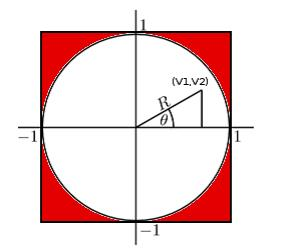
\includegraphics[width=6cm]{cercle}
	\centering
\end{figure}

Preuve:
A l'étape 4, Si $S<1$, le point $(V_1, V_2)$ est un point uniforme dans le cercle unité. Maintenant si on transforme en coordonnées polaires:
\[V_1 = R \cos{\Theta}\]
\[V_2 = R \sin{\Theta}\]

on trouve alors \[S = V_1^2+V_2^2 = R^2\]
\[X_1 = \sqrt{\frac{-2\ln{(S)}V_1^2}{S}} = \sqrt{\frac{-2\ln{(S)R^2\cos^2{\Theta}}}{R^2}} = \sqrt{-2\ln{S}}\cos{\Theta}\]
\[X_2 = \sqrt{\frac{-2\ln{(S)}V_2^2}{S}} = \sqrt{\frac{-2\ln{(S)R^2\sin^2{\Theta}}}{R^2}} = \sqrt{-2\ln{S}}\sin{\Theta}\]
\vspace{0.3cm}

On pose $R'=\sqrt{-2\ln{S}}$ et $\Theta' = \Theta$, on a donc $X_1=R'\cos{\Theta'}$ et $X_2=R'\sin{\Theta'}$. Il est évident que $R'$ et
$\Theta'$ sont indépendant car $R$ et $\Theta$ sont indépendants dans le cercle unité. Aussi, on a que 
\begin{itemize}
 \item $\Theta'$ est uniformément distribué entre 0 et $2\pi$
 \item $P(R'\leq r) = P(-2\ln(S)\leq r^2)$ = $P(S\geq e^{\frac{-r^2}{2}}) = 1-e^{\frac{-r^2}{2}}$ car $S=R^2$ est uniformément distribué entre
 0 et 1.
\end{itemize}

La probabilité que $R'$ se trouve entre $r$ et $r+dr$ est donc la dérivée de $1-e^{\frac{-r^2}{2}}$, à savoir $re^{\frac{-r^2}{2}}$.

De la même façon, la probabilité que $\Theta'$ se trouve entre $\theta$ et $\theta+d\theta$ est $(\frac{1}{2\pi})d\theta$.
\vspace{0.3cm}

La probabilité jointe que $X_1\leq x_1$ et $X_2\leq x_2$ peut maintenant être calculée de la façon suivante:

\begin{align}
 \int_{\{(r,\theta)|r \cos{\theta} \leq x_1, r\sin{\theta} \leq x_2\}} \frac{1}{2\pi}e^{-\frac{r^2}{2}}r\ dr\ d\theta
 & = \frac{1}{2\pi}\int_{\{(x,y)|x \leq x_1, y \leq x_2\}}e^{-(x^2+y^2)/2}dx\ dy \nonumber\\
 & = \left(\sqrt{\frac{1}{2\pi}} \int_{-\infty}^{x_1} e^{\frac{-x^2}{2}}dx \right)\left(\sqrt{\frac{1}{2\pi}} \int_{-\infty}^{x_2} e^{\frac{-y^2}{2}}dy \right) \nonumber
\end{align}
\vspace{0.3cm}

Ceci prouve que $X_1$ et $X_2$ sont indépendants et distribués selon une loi normale.
